%1
\documentclass[a4paper,11pt]{article}
\pdfoutput=1 % if your are submitting a pdflatex (i.e. if you have
             % images in pdf, png or jpg format)

\usepackage{jinstpub} % for details on the use of the package, please
                     % see the JINST-author-manual
\usepackage{lineno}
\usepackage{epstopdf}
\usepackage{wrapfig}

\title{\boldmath A search for Lepton Flavor Violating Decays of the Higgs Boson }
\proceeding{Oral Candidacy Exam proposal:\\
  Dated 19th of March, 2017\\
  }


%% %simple case: 2 authors, same institution
%% \author{A. Uthor}
%% \author{and A. Nother Author}
%% \affiliation{Institution,\\Address, Country}

% more complex case: 4 authors, 3 institutions, 2 footnotes
\author[a]{Nabarun Dev}

% The "\note" macro will give a warning: "Ignoring empty anchor..."
% you can safely ignore it.

% The "\note" macro will give a warning: "Ignoring empty anchor..."
% you can safely ignore it.

\affiliation[a]{Department of physics, University of Notre Dame, Indiana, USA}

% e-mail addresses: only for the forresponding author
\emailAdd{nabarun.dev@cern.ch, ndev@nd.edu}

\notoc
\compress
%\toccont
\abstract{A proposal is presented here outlining the search for lepton flavor violating (LFV) decays of the Higgs boson using the CMS experiment at the LHC. This a search for physics beyond the standard model and is performed with events where the Higgs decays to a muon and a tau lepton with the tau further decaying to an electron. The signal for which we are searching, the backgrounds and the experimental techniques used to discrimate signal from background are outlined in this proposal.}





\begin{document}
%\setpagewiselinenumbers
\linenumbers

\maketitle
\flushbottom

\section{Introduction}
\label{sec:intro}
%For internal references use label-refs: see section~\ref{sec:intro}.
The Standard Model (SM) of particles physics is the most well-tested and elegant description of nature available today. 
The discovery of the Higgs Boson in 2012 ~\cite{a} added another feather in the hat of the SM.
In the SM, elementary particles acquire mass from their interaction with the scalar Higgs field, the quantum of which is the  Higgs Boson.
Besides confirming the above mechanism by which particles acquire mass, the above discovery is also significant beause the Higgs provides a portal for us to not only further study the processes within the SM, but also to look for new physics processes beyond it (BSM). 
One of the main goals of the LHC  physics programme at CERN is to search for such BSM processes.


Lepton flavour violating (LFV) interactions between charged leptons cannot naturally occur within the standard model and such a process has never been observed experimentally.
However, such decays are allowed in many BSM theories such as models with more than one Higgs doublet ~\cite{b}, supersymmetric models ~\cite{c} and many others. 
Such interactions could thus be an indicator of new physics and could be realized in decays of the Higgs Boson into two charged leptons of different flavor.
Indirect constraints on LFV Higgs decays exists through interpretations of measurements of processes such as $\tau \rightarrow \mu \gamma ; \mu \rightarrow e \gamma$ ~\cite{d}~\cite{e}. 
These constraints set weak limits on LFV Higgs decays allowing significant branching fractions;$Br(H\rightarrow \mu \tau)<O(10\%).$
 A search for $H\rightarrow \mu \tau$ performed with data collected by the CMS during run I of the LHC  improved the above limits by an order of magnitude to $Br(H\rightarrow \mu \tau)<O(1.51\%).$ at 95\% confidence level. Also, an excess of events with a significance of 2.4$\sigma$ was observed. This warrants us to do this search with much larger amount of data which would either lead us to confirm this excess or squash it and set much stricter limits on this process. The run II of LHC (see section ~\ref{sec:lhccms})  provides us with such an opportunity to perform the search outlined in the following.   



\section{LHC and the CMS}
\label{sec:lhccms} 
The Large Hadron Collider (LHC) is a circlar particle accelerator designed to collide proton beams with a centre-of-mass energy of 14 TeV. It consists of a 27-kilometre ring of superconducting magnets with a number of accelerating structures to boost the energy of the particles along the way. Currently, (run II) the LHC operating at a COM energy of 13 TeV (compared to 7 TeV in run I) and luminosities up to $1.5 \times 10^{34} \mathrm{cm^{-2}s^{-1}}$. Under run II conditions, the Higgs production cross-section is a factor 2 higher~\cite{f} than run I (see figure~\ref{fig:a}) and almost twice the amount of dta has already been collected.     

\begin{figure}[htbp]
\centering
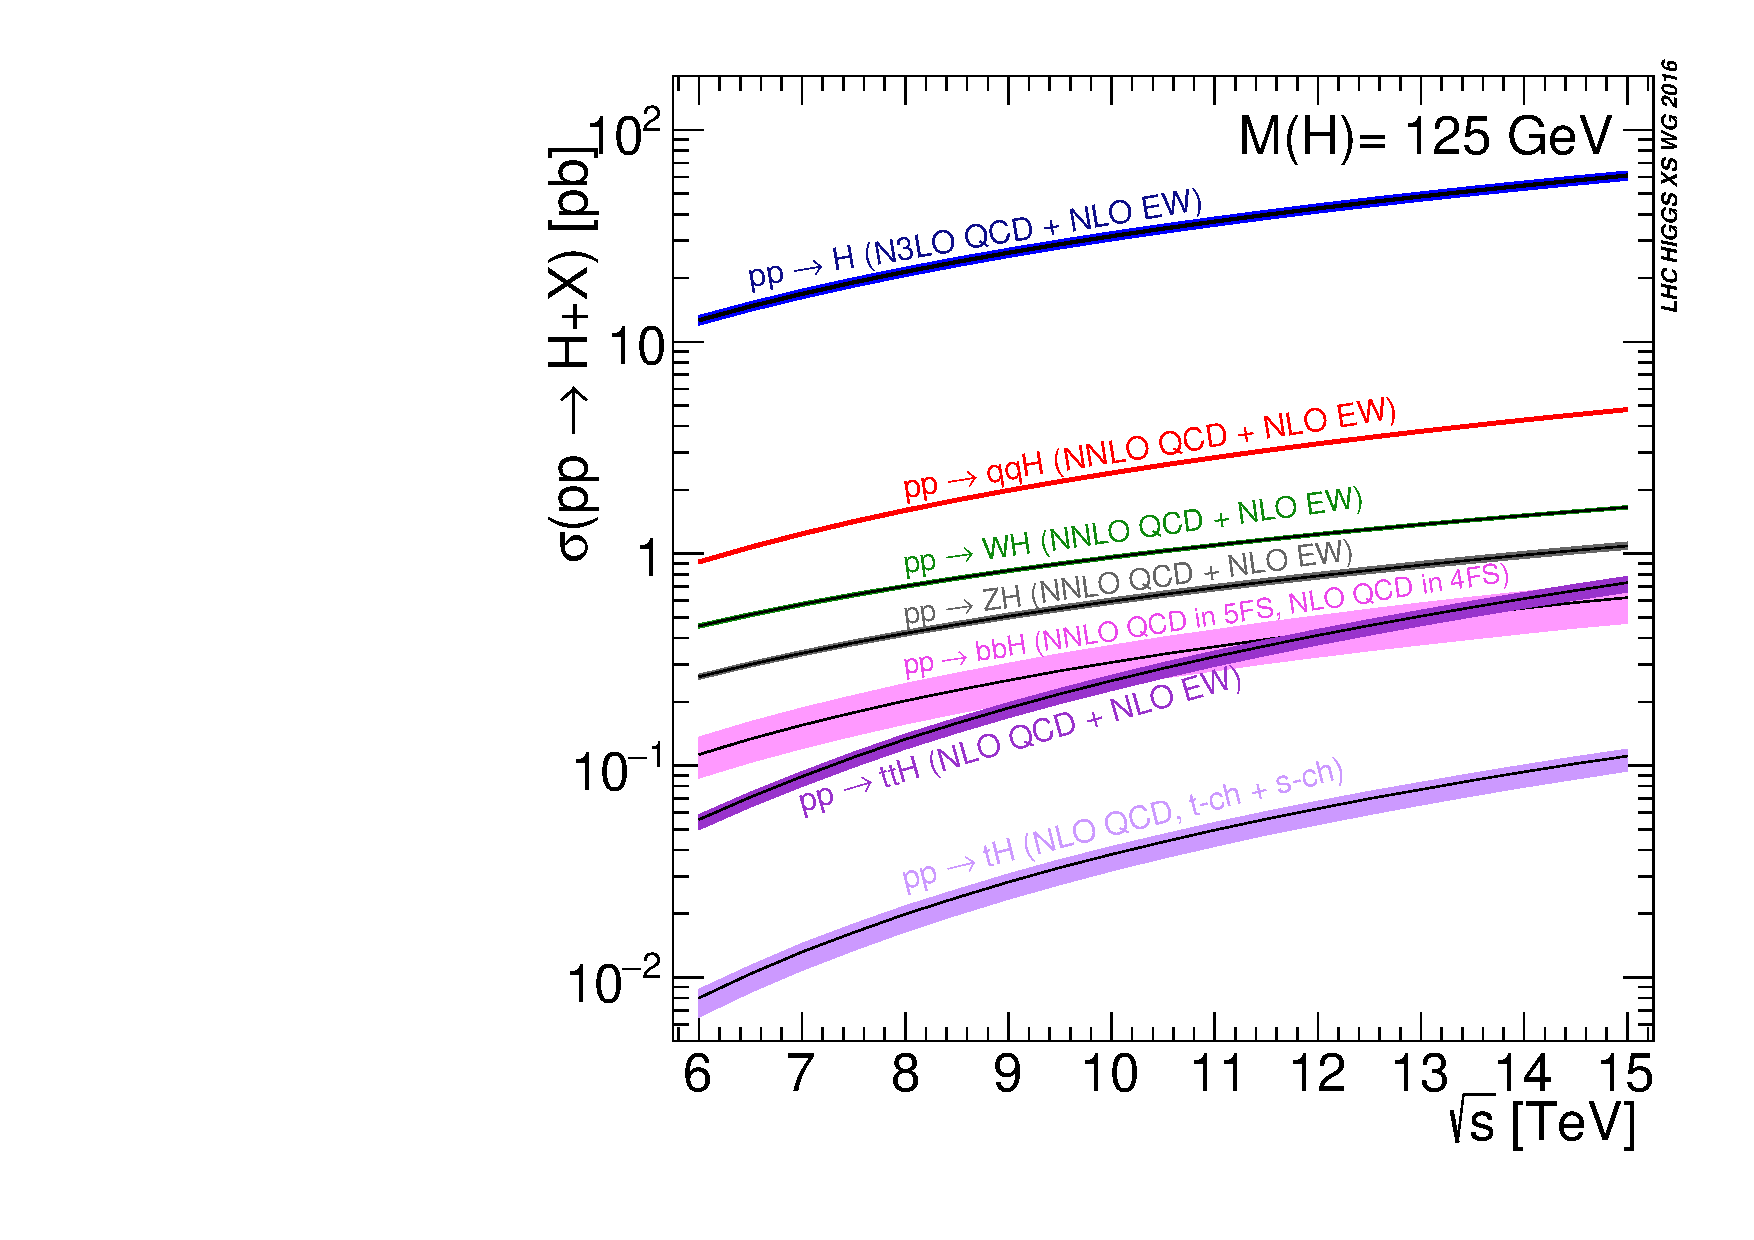
\includegraphics[width=.40\textwidth]{Plot_Escan_H125_new_sqrt.pdf}
\qquad
% "\includegraphics" from the "graphicx" permits to crop (trim+clip)
% and rotate (angle) and image (and much more)
\caption{\label{fig:a} Higg production cross-section as a function of the collison center-of-mass energy  }
\end{figure}

The Compact Muon Solenoid (CMS) is a large general purpose particle physics  detector  designed to study proton-proton collisions produced by LHC. 
\begin{wrapfigure}{r}{0.5\textwidth}
  \centering
    \includegraphics[width=.46\textwidth]{cms.png}
  \caption{\label{fig:b} The CMS detector  }
\end{wrapfigure}
A detailed description of the CMS detector can be found here~\cite{g}.
It consists of a superconducting solenoid that houses tracking and calorimetry systems and provides an axial magnetic field of 3.8T.The inner-most layer is the silicon pixel and strip tracker that measures the trajectories of charge particles and covers a range of $|\eta|<2.5$($\eta$ is the pseudorapidity defined as $-ln[tan(\frac{\theta}{2})]$, where $\theta$ is polar angle of the particle's trajectory with respect to the beam direction). Surrounding the tracker are the lead tungstate crystal electromagnetic calorimeter (ECAL) which measures the energy of electrons and photons, and the hadronic calorimeter (HCAL) which measure the energy of heavier particles that pass through the HCAL. The ECAL also contains preshower detector for extra spatial precision.Outside the solenoid is the muon system which has gas-ionization detectors placed in the steel yoke of the magnet. This is the outermost component of CMS and measures the momenta of muons that traverse through it.

Another vital component of the CMS is its trigger system. Only a small fraction of events produced by the LHC can be permanently stored, and to select these events of interest, CMS employs a sophisticated two-level trigger , organized in consecutive stages- the Level-1 (L1) trigger and the High Level Trigger (HLT). The L1 trigger is implemented using custom hardware and makes decisions based on coarse information from the calorimeters and the muon systems, reducing the rate from 40 MHz to 100 kHz. It has a latency of ~3.8$\mu$s. The software-based HLT partially reconstructs the event, implementing complex selection algorithms on finer granularity information from all sub-detectors in regions deemed interesting by the L1 decision. It runs on a massive computer farm and brings down the rate further to less than 1.5 kHz. I am part of a team that works on the cusp of ECAL and L-1 trigger and have helped maintain and improve the functioning of this system. This is mentioned in detail in section~\ref{sec:intro}.


\section {Overview of the Analysis}
\subsection{LFV Signal}
In BSM theories it is possible to introduce off-diagonal Higgs-fermion Yukawa couplings such as $Y_{\mu\tau}$ in addition to the SM $Y_{\mu\mu}$,$Y_{\tau\tau}$,$Y_{ee}$ couplings allowing the Higgs to decay into to oppositely charged leptons of different flavor.  The decay studied here $H\rightarrow \mu\tau$ with that $\tau$ decaying to an electron (and neutrinos) is of particular importance because CMS can much better identify and reconstruct an electron than a hadronically decaying tau making for a cleaner signature. It is important to note that $H\rightarrow \mu\tau_{e}$ final state bears some similarities with SM $H\rightarrow \tau_{\mu}\tau_{e}$ process albeit with significant kinematic differences.
\begin{wrapfigure}{r}{0.5\textwidth}
  \centering
    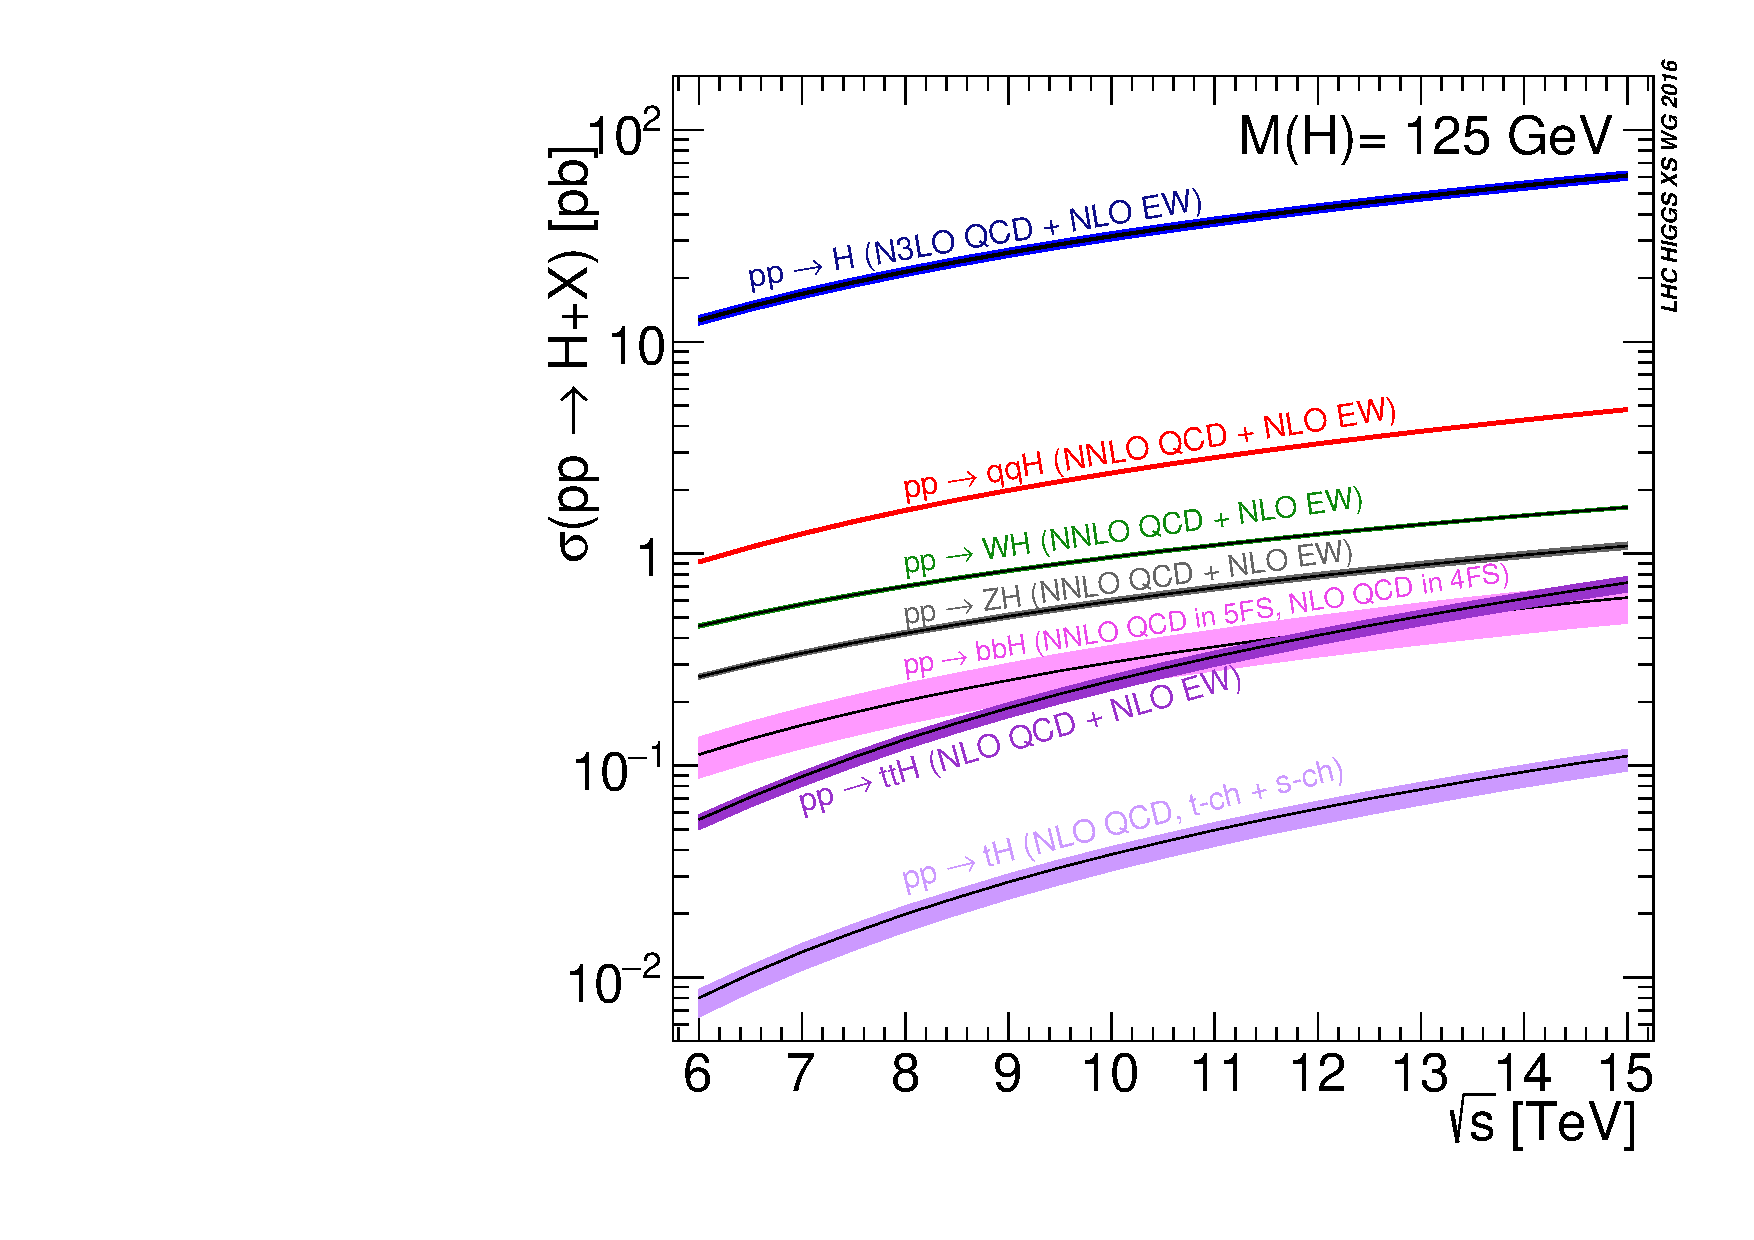
\includegraphics[width=.46\textwidth]{Plot_Escan_H125_new_sqrt.pdf}
  \caption{\label{fig:c} Higg production cross-section as a function of the collison center-of-mass energy  }
\end{wrapfigure}

The muon in the LFV decay comes promptly from the H and has a harder $p_{T}$ spectrum compared to the SM muon. There are fewer neutrinos in the LFV decay which makes its missing transverse ($E_{T}^{miss}$) energy spectrum (neutrinos being very weakly interacting can't be detected by CMS and their transverse momenta can be estimated from $E_{T}^{miss}$). Further, the neutrinos in the LFV process come from the decay of the highly boosted tau, leading the $E_{T}^{miss}$ and electron to be highly collinear. This fact also motivates us to use collinear mass ($M_{coll}$) as an estimator of the reconstructed H mass. This is based on the collinear approximation~\cite{h}- the mass of the H being much greater than the mass of the $\tau$, all the $\tau$ decay products are boosted in the direction of the $\tau$. The neutrino momenta ($p_{T}^{\nu,~\text{est}}$) can thus be approximated to be in the same direction of the electron and can be estimated form the projection of $E_{T}^{miss}$ onto the $\tau$ direction.The collinear mass can then be derived from the visible mass of the $\tau$-$e$ system ($M_{\text{vis}}$) as $M_{\text{col}}= M_{\text{vis}} / \sqrt{x_{\tau}^\text{vis}}$, where $x_{\tau}^\text{vis}$ is the fraction of energy carried by the visible decay products of the $\tau$ ($x_{\tau}^\text{vis}={p_{T}^{\tau^{\text{vis}}}}/{(p_{T}^{\tau^\text{vis}}+p_{T}^{\nu,~\text{est}})}$).

\subsection{Background processes}

\begin{figure}[htbp]
\centering % \begin{center}/\end{center} takes some additional vertical space
\includegraphics[width=.47\textwidth, ]{isolation.pdf}
\qquad
\includegraphics[width=.47\textwidth, ]{clusters.png}
% "\includegraphics" from the "graphicx" permits to crop (trim+clip)
% and rotate (angle) and image (and much more)
\caption{\label{fig:k} Left: Illustration of dynamic clustering of TTs and e/$\gamma$ isolation region (blue) with the exclusion of footprints in ECAL and HCAL. Right: Various cluster shapes from dynamic clustering. Smaller e/$\gamma$-like clusters are shown on top and larger jet like clusters are shown below.}
\end{figure}


These algorithms were developed using Run I data and simulated Run II data. Their performance was then validated using data taken in 2015 during the commissioning period of the new trigger system, and they exhibit much superior performance compared to the Run I trigger. The position resolution is better by  a factor of 4 and the energy resolution has improved by up to 30\% with respect to Run I~\cite{h}. In particular, the energy resolution in the EE is now improved and closer to that in the EB. This is due to dynamic clustering being very well adapted to the complex geometry of EE. Further, the efficiency is also better with sharper turn-on curves accompanied by a reduction in rate.

\subsection{Firmware implementation}
The algorithms are implemented in the firmware using the VHDL  hardware description language. The  firmware for the electron finder along with the tau lepton and jet finders must fit within a single Xilinx FPGA, which makes its implementation a challenge. In addition, the core firmware, which comprises all necessary logic to control the I/O optical serial links, the configuration registers, the input pattern buffers, output spy buffers are also included. As seen in Figure~\ref{fig:floorplan}, a precise floor planning scheme was developed to efficiently perform a place and route process, and to guarantee that timing constraints are satisfied after modification of  VHDL sources during the development process. An internal processing speed of 240 MHz has been achieved with this approach. About 65\% of the logic resources of the chip are being used, which include the electron/photon, jet, tau lepton and missing E$_\text{T}$ triggers. The software interface is based on the IPBUS standard using libraries such as $\mu$HAL developed at CERN~\cite{e}.
\begin{figure}[!htbp]
\begin{center}
\begin{minipage}[t]{7cm}
\begin{center}
\vspace{0cm}
\includegraphics[angle=90,width=6.8 cm, trim=3cm 0cm 0cm 0cm]{Layer2Firmware.png}
\end{center}
\end{minipage}
\hspace{1cm}
\begin{minipage}[t]{6cm}
\begin{center}
\caption{ \label{fig:floorplan}Floor planning of Xilinx Virtex 7 FPGA within the MP7 board. The purple areas represent the input-output logic within the core firmware and the yellow represents the resources used by the algorithms. The red corresponds to the DAQ interface and the green the IPBus that handles the communications. }
\end{center}
\end{minipage}
\end{center}
\end{figure}
The TMT architecture allows for data coming from calorimeters to be rearranged in geometrical order~\cite{f}. Algorithms are fully pipelined (spatially) and process data at the incoming rate starting on the reception of the first data word. The TTs are combined to form basic blocks of 3$\times$1 TTs (see section~\ref{subsec:cmstriggerecal}) upon reception. These are further combined to form bigger blocks which are the input components of algorithms. Potential cluster seeds are identified depending on the TT energy threshold. Quality flags are also set for each incoming TT based on several predefined selection criteria and help in reducing the number of resources required for the implementation of lepton cluster logic. The fully pipelined firmware approach provides an efficient way to localize the processing, reduce the size and number of fan-outs, minimize routing delays and eliminates register duplication leading to a compact and easily maintainable firmware.

 
\section{Performance of the upgraded e/$\gamma$ trigger in 2016}
The new L1 trigger system was commissioned in September 2015 and has been used for physics throughout data taking in 2016, and has delivered very good performance from the start. Its performance has remained excellent with the LHC delivering data at increasingly higher luminosities with higher pileup levels. The performance of the trigger in 2016 CMS physics data taking is shown in Figures 5, 6 and 7. The position resolution of the new trigger system in 2016 is presented in Figure~\ref{fig:l}. This was computed with respect to offline electron superclusters (these are clusters produced by offline electron reconstruction algorithms) using $Z\rightarrow ee$ events in 13 TeV data recorded in 2016. These plots illustrate excellent spatial resolution provided by the new trigger.
The energy resolution of the L1 trigger is shown in Figure~\ref{fig:m}. This was computed with respect to transverse energy of the offline electron superclusters using $Z\rightarrow ee$ events. A geometrical matching between the electron supercluster and the L1 candidate is applied. The energy resolution delivered is excellent in all $\eta$ ranges. 
In terms of trigger efficiency, turn-on curves for 2016  $Z\rightarrow ee$ data, evaluated using tag-and-probe techniques are shown in Figure~\ref{fig:n}. The sharp turn-on curves and high trigger efficiency are due to the excellent energy resolution and the performance of the new clustering algorithms. These sharp turn-on curves allow CMS to maintain low thresholds on physics object selection. 

\begin{figure}[htbp!]
\centering % \begin{center}/\end{center} takes some additional vertical space
\includegraphics[width=.45\textwidth]{plottopleft.png}
\qquad
\includegraphics[width=.45\textwidth]{plottopright.png}
% "\includegraphics" from the "graphicx" permits to crop (trim+clip)
% and rotate (angle) and image (and much more)
\caption{\label{fig:l}Differences in pseudo-rapidity $\eta$ (left) and azimuthal angle $\phi$ (right) for L1 EG candidates with respect to the
offline reconstructed electron supercluster, in the barrel (|$\eta$|<1.479, in black) and in the endcaps (|$\eta$| >1.479, in red)} 
\end{figure}

\begin{figure}[htbp!]
\centering % \begin{center}/\end{center} takes some additional vertical space
\includegraphics[width=.45\textwidth]{plotmiddle.png}
\qquad
% "\includegraphics" from the "graphicx" permits to crop (trim+clip)
% and rotate (angle) and image (and much more)
\caption{\label{fig:m}Relative difference in transverse energy for L1 EG candidates with respect to the offline reconstructed transverse energy, in the range 0$\leq$|$\eta$|<0.25 (black), 1$\leq$|$\eta$|<1.25 (red) and 2$\leq$|$\eta$|<2.25 (blue)}
\end{figure}

\begin{figure}[htbp!]
\centering % \begin{center}/\end{center} takes some additional vertical space
\includegraphics[width=.44\textwidth]{plotbottomleft.png}
\qquad
\includegraphics[width=.44\textwidth]{plotbottomright.png}
% "\includegraphics" from the "graphicx" permits to crop (trim+clip)
% and rotate (angle) and image (and much more)
\caption{\label{fig:n}Left: L1 trigger efficiency for an e/$\gamma$ object as a function of the offline reconstructed supercluster transverse energy E$_\text{T}$ for electrons in the barrel (|$\eta$|<1.479, in black) and in the endcaps (|$\eta$|>1.479, in red), for a threshold of 24 GeV (left) with and for a threshold of 40 GeV (right) without isolation requirement.}
\end{figure}

\section{Conclusions}

The upgraded calorimeter trigger has been running smoothly from the start of data taking in 2016 and has exhibited excellent performance. The isolation criteria and energy calibration are optimized at regular intervals to follow the increasing LHC luminosity which currently peaks at more than $1.5 \times 10^{34} \mathrm{cm^{-2}s^{-1}}$. The new trigger has enabled CMS to maintain low e/$\gamma$  thresholds throughout LHC Run II. The current trigger scheme for physics includes: single isolated and non-isolated e/$\gamma$  triggers for electroweak (EWK) processes; double e/$\gamma$, triple e/$\gamma$ triggers for Higgs physics. It is possible for CMS to increase its selectivity by introducing new invariant mass triggers for EWK processes. The new trigger architecture, being modular, provides the flexibility to add more processing nodes if needed. It is very important for the e/$\gamma$ trigger to be able to perform efficiently to be maximally sensitive to new physics signatures over a wide range of particle energies. The new CMS Level-1 electron and photon trigger has delivered very high performance in 2016, consistent with expectations and is expected to do so throughout challenging conditions of LHC Run II and Run III.    
  
\begin{thebibliography}{}

\bibitem{a}CMS Collaboration, \emph{The CMS Experiment at the CERN LHC}, \emph{JINST} {\bf 3 S08004} (2008) .
\bibitem{b}CMS Collaboration, \emph{CMS TriDAS project: Technical Design Report, vol. 1: The Trigger Systems
}, \emph{CERN-LHCC-2000-038}, {\bf  CMS-TDR-6-1} (2000) .
\bibitem{c}CMS Collaboration, \emph{CMS Technical Design Report for The Level-1 Trigger Upgrade}, \emph{CERN-LHCC-2013-011} {\bf CMS-TDR-12} (2008).
\bibitem{d}A. Zabi for CMS collaboration\emph{The CMS Level-1 Calorimeter Trigger for LHC Run II}, \emph{these proceedings } {\bf TWEPP } (2016).
\bibitem{e}T. Williams et al., \emph{IPbus:  A  flexible  Ethernet-based  control  system  for  xTCA  hardware}, \emph{JINST} {\bf 10 C02019} (2015).
\bibitem{f}A. Zabi for CMS Collaboration, \emph{Triggering on electrons, jets and tau leptons  with the CMS upgraded calorimeter trigger for
the LHC RUN II}, \emph{JINST} {\bf 11 C02008} (2016).
\bibitem{g}J.B. Sauvan for CMS Collaboration \emph{Performance and upgrade of the CMS electron and photon trigger for
Run 2}, \emph{J. Phys. Conf. Ser.} {\bf 587} (2015) 012021.
\bibitem{h}T. Strebler for CMS Collaboration, \emph{Level-1 trigger selection of electrons and photons with CMS for LHC Run-II}, \emph{CMS CR} {\bf -2015/220} (2008) .
 

% Please avoid comments such as "For a review'', "For some examples",
% "and references therein" or move them in the text. In general,
% please leave only references in the bibliography and move all
% accessory text in footnotes.

% Also, please have only one work for each \bibitem.


\end{thebibliography}
\end{document}
